\chapter{Počítačový hráč}
\section{Tahová logika}
Hráče na desce bychom si mohli rozdělit do dvou skupin v závislosti na nejrelevantnějších osách určujících jejich směr pohybu. U hráčů v nejnižším a nejvyšším cípu hvězdy (tedy v právě těch dvou cípech, které jsou využívány při hře dvou hráčů) je nejrelevantnější $y$-ová osa. Cílem těchto hráčů je totiž cíp mající polohu na $x$-ové ose shodnou s jejich výchozím cípem, a proto není důležitost polohy jejich tahů na $x$-ové ose příliš velká. U zbývajících čtyř hráčů toto ale neplatí vzhledem k~tomu, že jejich cílové cípy mají kromě odlišné polohy na $y$-ové ose odlišnou také polohu na $x$-ové ose. Pro tyto čtyři hráče je tedy velmi důležitá také poloha jejich tahů na $x$-ové ose. Z tohoto důvodu je implementace vykonávání pohybů pro obě tyto skupiny hráčů do značné míry odlišná. U popisu chování hráče proto vykonávaní pohybů pro obě tyto skupiny popisujeme odděleně. Názorná ukázka směrů, kterým hráči táhnou s ohledem na $x$-ové a $y$-ové souřadnice je na obrázku číslo \ref{fig:SmeryTahu}.

\begin{figure}
	\centering
	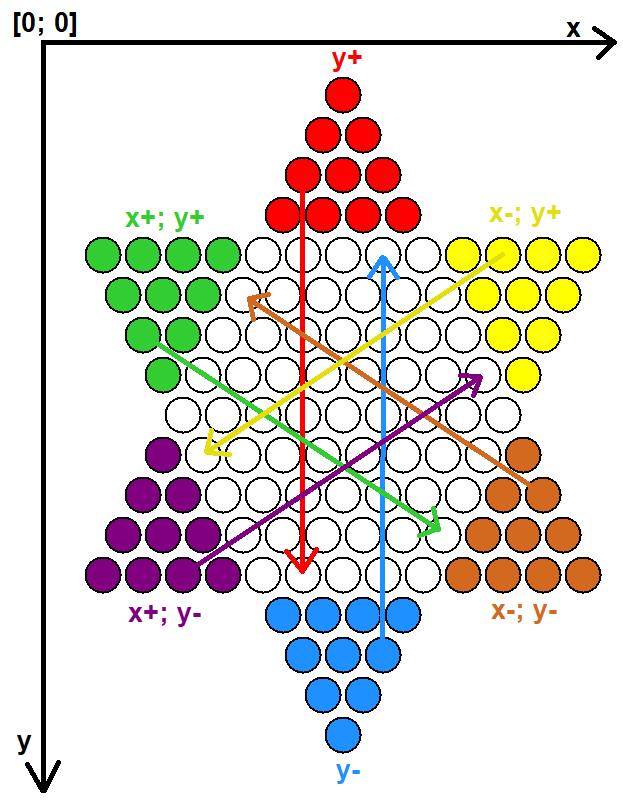
\includegraphics[width=0.7\textwidth]{Figures/SmeryTahu.png}
	\caption{Směry tahů hráčů s ohledem na $x$-ové a $y$-ové souřadnice}
    \label{fig:SmeryTahu}
\end{figure}

Existují ale i tahy, u kterých není okamžitá uražená vzdálenost nejdůležitějším parametrem. Asi nejtypičtějším příkladem takových tahů jsou prvotní tahy, tedy tahy vykonávané na začátku hry. V~ této práci je implementován prvotní tah Cross Caterpillar, jehož princip je vysvětlen v~podkapitole \ref{sec:Strategie}. Od klasických tahů se odlišují také tahy vykonávané na úplném konci hry. Na konci hry je totiž velmi vysoká pravděpodobnost, že kameny počítačového hráče jsou rozmístěny takovým způsobem, že je nutné provést tahy neodpovídající směrům uvedeným v obrázku číslo \ref{fig:SmeryTahu}. Příklad takové situace můžeme zhlédnout na obrázku číslo \ref{fig:SituaceNaKonciHry}. Odděleně implementované prvotní a koncové tahy ale nejsou vzhledem k existenci různých obtížností počítačových hráčů využívány vždy, využití těchto tahů je detailně rozebráno v následující podkapitole týkající se právě obtížností počítačových hráčů.

\begin{figure}
	\centering
	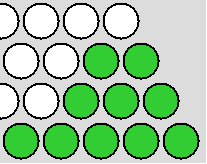
\includegraphics[width=0.4\textwidth]{Figures/SituaceNaKonciHry.png}
	\caption{Příklad situace na konci hry, kdy hráč musí provést tah v jiném než určeném směru}
    \label{fig:SituaceNaKonciHry}
\end{figure}

Dále je nutné při tazích počítačového hráče brát v potaz lidského hráče. Konkrétně je nutné zvažovat, jak provedení tahu počítačového hráče ovlivní lidského hráče. Je totiž dost pravděpodobné že během hry dojde k situaci, kdy počítačový hráč provede pro něj nejvýhodnější tah, jehož vykonání ale dá lidskému hráči možnost provést výhodnější tah, než jaký mohl provést před vykonáním tahu počítačového hráče. K zabránění vykonání takového tahu slouží metoda \lstinline$JeTahVyhodny$ ve třídě \lstinline$PohybPocitacovehoHrace$, která provede simulaci vykonání tahu počítačového hráče a zjistí, jestli může po jeho vykonání lidský hráč provést výhodnější tah než předtím. Metoda ale není využita vždy, stejně jako u předchozího odstavce i zde její využití závisí na obtížnosti počítačového hráče, využití je tedy popsáno v následující podkapitole.

Při tahu může nastat situace, kdy není možné provést žádný logický tah odpovídající směrům uvedeným na obrázku číslo \ref{fig:SmeryTahu}. Typicky může taková situace nastat při hře 6 hráčů ke konci hry, kdy už zbývá hráči do cílového trojúhelníku přesunout pouze několik kamenů, přičemž cesta je blokována kameny ostatních hráčů. V takovém případě je proveden náhodný tah, táhne se vždy ale pouze s některým z kamenů, který zatím není v cílovém trojúhelníku. 

\section{Úrovně obtížnosti}
\label{sec:UrovneObtiznosti}
Při vytváření her, ve kterých lidský hráč bojuje proti počítačovým hráčům, je jedním z hlavních cílů vytvořit lidskému hráči rovnocenného, tedy co nejsilnějšího protivníka. Je ovšem také nutné brát v~potaz rozdílné dovednostní úrovně lidských hráčů -– začátečník jistě nebude ve hře tak dobrý jako zkušený hráč. Z tohoto důvodu jsou v této hře implementovány tři různé obtížnosti počítačových nepřátel. Před začátkem hry pak lidský hráč nastaví obtížnost jeho počítačových nepřátel.

Nejprve rozebereme počítačového hráče s nejnižší úrovní obtížnosti, dále bude označován jako \emph{lehký}. U hráčů v nejvýše a nejníže položeném trojúhelníku je během každého tahu proveden pohyb, který je neposune směrem opačným vzhledem k jejich cíli na $y$-ové ose. Jinak řečeno, kámen musí být během tahu posunut blíže k cíli, nebo musí zůstat stejně daleko (týká se pouze $y$-ové osy, na $x$-ovou osu není brán zřetel). U zbývajících čtyř hráčů je pak nutné, aby byl tah veden~v~obou směrech znázorněných na obrázku číslo \ref{fig:SmeryTahu}. Například kámen zeleného hráče musí být vždy přemístěn do pole, které má vyšší $x$-ovou i $y$-ovou souřadnici než samotný kámen. Není vybírán nejvýhodnější tah, z možných tahů splňujících zmíněnou podmínku je vždy náhodně vybrán jeden z nich.

Další je počítačový hráč s vyšší úrovní obtížnosti, ten bude dále označován jako \emph{střední}. Ten funguje na podobném principu jako lehký hráč, z proveditelných tahů je také vždy vybrán jeden z~nich, liší se v podmínkách proveditelnosti tahů. U hráčů v nejvýše a nejníže položeném trojúhelníku je nutné, aby byl kámen během tahu posunut blíže k cíli na $y$-ové ose. Proti lehkému hráči se liší v tom, že kámen nemůže během tahu zůstat na $y$-ové ose stejně daleko k cíli. U zbývajících čtyř hráčů je pak nutné, aby byl tah veden v alespoň jednom ze směrů uvedeném na obrázku číslo \ref{fig:SmeryTahu}. Kámen zeleného hráče musí tedy být přemístěn do pole, které má vyšší buď $x$-ovou, nebo $y$-ovou souřadnici. Mohlo by se zdát, že je kvůli tomuto rozdílu střední hráč slabší než lehký hráč, ale není tomu tak. Lehký hráč sice projde herní deskou rychleji, znatelný rozdíl ale nastane v závěrečné fázi hry -– zatímco střední hráč své kameny rozloží rovnoměrně do celého cílového trojúhelníku, lehký hráč nejdříve obsadí okraje sousedící s nejvýše nebo nejníže položeným trojúhelníkem (v závislosti na poloze cílového trojúhelníku). Kvůli tomu lehký hráč potřebuje k dokončení hry mnohem větší počet tahů než střední hráč.

Posledním nezmíněným hráčem je počítačový hráč s nejvyšší úrovní obtížnosti, dále bude označován jako \emph{těžký}. Tento hráč se od lehkého i středního hráče velmi zásadně liší. Během každého tahu je vždy proveden nejvýhodnější možný pohyb, jeho tahy tedy nikdy nejsou náhodné. U hráčů v nejvýše a nejníže položeném trojúhelníku je vždy proveden tah, který hráče posune co nejblíže k cíli na $y$-ové ose. V potaz je zde ale brána i $x$-ová osa -– z tahů nejvýhodnějších podle $y$-ové osy je proveden ten z nich, který hráče posune nejblíže k středu mapy. U zbývajících hráčů je pak proveden tah, který je dostane nejdál ve směru uvedeném v obrázku číslo \ref{fig:SmeryTahu}. U hráčů v nejvýše a nejníže položeném trojúhelníku je prováděn počáteční tah Cross Caterpillar (u zbývajících hráčů prováděn není vzhledem k tomu, že jeho provedení u nich ve výsledku zvýší počet tahů potřebný pro vítězství). U všech hráčů s touto obtížností jsou také ošetřeny koncové tahy, což výrazně sníží počet tahů potřebných k vítězství. Je zde taktéž kladen důraz na možné budoucí tahy lidského hráče, pro tyto účely je využívána metoda \lstinline$JeTahVyhodny$ popsaná v předchozí podkapitole.

Výpis všech relevantních dovedností a schopností jednotlivých počítačových hráčů podle jejich obtížnosti se nachází v tabulce číslo \ref{tab:ObtiznostiPocitacovychHracu}.

\begin{table}
	\centering
	\caption{Dovednosti a vlastnosti počítačových hráčů podle obtížnosti}
	\label{tab:ObtiznostiPocitacovychHracu}
	\begin{tabular}{cccc}
		\toprule
		Vlastnost & \multicolumn{1}{c}{Lehký} & \multicolumn{1}{c}{Střední} & \multicolumn{1}{c}{Těžký}\\
		\midrule
		Zajištěna výhra v rozumném počtu tahů & \faTimes & \faCheck & \faCheck\\
		Náhodné pohyby & \faCheck & \faCheck & \faTimes\\
		Vykonání nejvýhodnějšího tahu & \faTimes & \faTimes & \faCheck\\
		Brán ohled na tahy lidského hráče & \faTimes & \faTimes & \faCheck\\
		Počáteční pohyby & \faTimes & \faTimes & \faCheck*\\
		Koncové pohyby & \faTimes & \faTimes & \faCheck\\
		\bottomrule
	\end{tabular}
	\begin{tablenotes}
      \small
      \item *U hráčů v nejvýše a nejníže položeném trojúhelníku
    \end{tablenotes}
\end{table}

\section{Simulátor}
Pro praktickou ukázku síly jednotlivých počítačových hráčů podle jejich obtížností je v aplikaci implementován simulátor. Ten je spravován samotným uživatelem, který si může navolit počet hráčů a obtížnosti jednotlivých hráčů. Tito hráči budou poté hrát proti sobě bez dalšího zásahu uživatele. 

Tyto simulace je možné provádět dvěma způsoby. Uživatel může buďto nechat provést simulaci o~daných parametrech pouze jednou, nebo může nechat provést větší množství simulací o daných parametrech po sobě. Dá se tedy říct, že druhý způsob slouží spíše k statistickým účelům než k~sledování průběhu konkrétní hry. Z toho důvodu je uživateli promítnut průběh hry a výsledek pouze během provádění jediné simulace. U obou způsobů provádění simulací je nicméně výsledek zaznamenán do souboru \textsf{Statistiky.txt}, který se nachází v kořenovém adresáři aplikace. Do záznamu je uložen počet hráčů, počet tahů, obtížnost jednotlivých hráčů a výsledek simulace. Uživatel může všechny uložené statistiky nalézt i v samotné aplikaci, jsou dostupné v hlavním menu po výběru možnosti \textsf{Statistiky}.

V této práci je simulátor využit pro ukázku dovedností počítačových hráčů podle jejich obtížností v kapitole \ref{sec:HryMeziPocitacovymiHraci}.
\endinput